\documentclass[11pt,a5paper]{book}
\usepackage[utf8]{inputenc}
\usepackage{amsmath}
\usepackage{amsfonts}
\usepackage{amssymb}
\usepackage{graphicx}
\usepackage[super]{nth}
\usepackage{float}

\title{One Fish, Two Fish}
\author{Marcel Gietzmann-Sanders}
\date{}
\setcounter{tocdepth}{1}
\begin{document}
\maketitle
\tableofcontents
\newpage
\chapter{How to Digest a Brick}

\section{Well What's the Point?}

Quantitative fisheries science (hereafter referred to just as fisheries modeling) is all about the following question:
\newline

\hangafter=0 \hangindent=1cm \noindent How can a fishery bring the most long term benefit to society?
\newline

Nice and clear, right? Hardly. This is one of those wonderfully simplistic statements that throws a veil of apparent clarity over an entangled mass of delicious complexity. In other words, there's a lot to unpack.
\newline

Like all such statements it takes only the most rudimentary of questions to blow its cover. For example - what is a fishery? That's a question biologists are still arguing about and in all likelihood we've been fishing since before the invention of fire itself! 
\newline

Fortunately humans are pretty good at pretending the world is a lot simpler than it is and somehow managing to get away with it. Abstraction is a rather powerful tool of ours.
\newline

That being said the fun in a question like this one is not the abstraction itself but in the mind opening richness that comes from unraveling it.
\newline

So let's do some unraveling shall we? 
\newpage

\noindent \rule{\textwidth}{0.5pt} 
\noindent How can a \textbf{fishery} bring the most long term benefit to society?
\newline
\rule{\textwidth}{0.5pt} 
\vspace{5pt}

I know what you're thinking. Didn't I just say that no one's actually been able to agree on what a fishery \textit{exactly} is? How on earth then do I suppose I'm about to answer the question myself? 
\newline

Well see, if I don't at least present a working definition... well... then we'll have nothing to work with and this whole exploration of fisheries science will be rather short. So consider this definition less of an audacious claim of certainty on my part and more of a desperate attempt to find some common ground for us to stand on. 
\newline

Alright, here goes. A fishery in this book is going to mean a specific group of marine populations, at least one of which we catch and use. This definition is nice because it allows for both ecosystem based management (multiple interacting populations) and more tradition forms of management that work with one species at a time. 
\newline

That being said it's worth noting that I'm looking at the population as a whole. And that means I'm roping in \textit{everyone} who touches it. Unintended catch (bycatch), intended catch, commercial, recreational, artisinal, I'm throwing them all in the same... well... boat. I think as we pull the thread and unravel this problem it will become clear why I've decided to do this, but just be warned that to others a fishery can mean quite the opposite. Instead of focusing on the population such definitions often focus on the humans fishing it. 
\newpage

\noindent \rule{\textwidth}{0.5pt} 
\noindent How can a fishery bring the most long term \textbf{benefit} to society?
\newline
\rule{\textwidth}{0.5pt} 
\vspace{5pt}

If defining a fishery was difficult, defining what benefit to society means is even more so. Which is why I'm just not going to bother.
\newline

At least not now.
\newline

Benefits to society are marvelously specific to the fishery in question. These boons can be nutritional, cultural, financial, ecological, spiritual... yea you get the idea. Fisheries can make or break communities, they provide medical inputs, represent a multi-billion dollar industry, provide a primary source of protein to a good half of the entire world population, and are, quite critically, an essential part of an unnerving proportion of my lunches (although I may be a bit biased on that last point).
\newline

My point is simple - benefits cannot be defined in the abstract, you have to get down and dirty to \textit{really} understand what a fishery does and what it can mean to society. 
\newline

\textit{Know thy fishery}.
\newpage


\noindent \rule{\textwidth}{0.5pt} 
\noindent How can a fishery bring the most \textbf{long term} benefit to society?
\newline
\rule{\textwidth}{0.5pt} 
\vspace{5pt}

The need for food is one of those things that just doesn't go away. No matter how many times you eat, no matter how excellent the food, you always end up hungry a few hours later. It's just life. As such fisheries have to be sustainable - they \textit{need} to be able to bring in food year after year after year. And this often leads to a pill that's hard to swallow - in order to not burn out one has to slow down. (And that's a bit of wisdom that applies to a lot more than just catching fish). \newline

Each and every fishery must sort out not just how to bring benefit but how to guarantee that benefit to all those who will inherent the earth.
\newpage


\noindent \rule{\textwidth}{0.5pt} 
\noindent How can a fishery bring the \textbf{most} long term benefit to society?
\newline
\rule{\textwidth}{0.5pt} 
\vspace{5pt}

This now, well this is the question that brings out the pitchforks, firebrands, and lobbyists. It's one thing to acknowledge all the benefits a fishery can bring to society - figuring out how to balance all of these value propositions is quite another thing. Beyond struggling with the question of who society is and how to make sure it is represented, this balancing act may be the single most important activity in fisheries management which is exactly why I'm not going to attempt to answer the question at all. 
\newline

I am not judge, jury, and executioner - I'm just a dude who likes fish, numbers, and environmental stewardship. But suffice it to say, fisheries scientists have a \textit{responsibility} to help ensure that the political conversation is as data driven as possible and help create win-win situations whenever possible. These kinds of things tend to pit folks against each other and arch-nemeses make for incredible blinders.
\newline

Just as importantly it's paramount that every fisheries scientist out there recognizes that while their science may seem impartial or whatever there is always an implicit balance of benefits in every single optimization we ever do. That's a hard truth one can never escape. Know what you're fighting for because any and all data represents ammunition for someone. 
\newpage

\noindent \rule{\textwidth}{0.5pt} 
\noindent \textbf{How} can a fishery bring the most long term benefit to society?
\newline
\rule{\textwidth}{0.5pt} 
\vspace{5pt}

Obviously there are loads of ways to improve the benefits to society. Finding better ways to fish, setting catch limits to prevent the merciless decimation of a fish stock, being smarter about what's taken and what's left to breed and grow - these are some of the more apparent ones. However there are loads of other ways to hack the value of fisheries - becoming a restaurateur who changes public opinion about a specific species of fish, developing monitoring for the supply chain to help people understand where their food is coming from, or finding new ways to farm fish - there are a lot of really cool and interesting options. 
\newline

However I know I've got limited time with you and so, for the sake of brevity, I'm going to have to limit scope. So we're going to focus on being creative about the actions the fishers themselves can take when they're out actually catching the fish. For the full range of ingenious action that can be taken I refer you to the rich literature surrounding fisheries. 
\newpage

\noindent \rule{\textwidth}{0.5pt} 
\noindent  How can a fishery bring the maximum long term benefits to \textbf{society}?
\newline
\rule{\textwidth}{0.5pt} 
\vspace{5pt}

This is a question with an obvious answer that probably should be paid more attention to. Society is \textit{all} of us. It's not just mega-corps, it's not just the town near the fish that's been fishing there for centuries, and its not limited to the consumer either. It is \textit{everyone} and making sure \textit{all} are represented is of utmost importance. 
\newline

And as with the "most" question each and every model we build, each optimization we run, has implicit notions about \textit{who} society is. Be conscientious of that. 
\newpage

Alright, with all of that in mind I think our question is looking a little bit different. 
\newline

\hangafter=0 \hangindent=1cm \noindent \textbf{Fisheries modeling is about informing the set of fishing practices that would maximize a specific balance of benefits in a sustainable fashion. This information should then be used as part of a representative collaboration to find the balance best suited to the whole.}
\newline

So, what's needed to make this happen? Well wouldn't you know? By a wonderful coincidence that just happens to be what the next section is about. 
\newpage

\section{The 30,000 Foot View}

\noindent \rule{\textwidth}{0.5pt} 
\begin{figure}[h!] 
  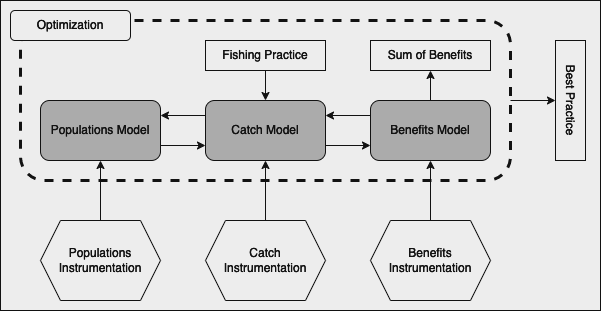
\includegraphics[width=\linewidth]{drawings/high_level_models.png}
  \caption{Models}
  \label{fig:high_level_models}
\end{figure}
\newline
\rule{\textwidth}{0.5pt} 
\vspace{5pt}

To optimize requires predicting things that have never happened (and likely never will). Doing so requires mathematical models that give you the confidence to wade into the unknown. And for our particular problem those models split into three broad categories - benefits, population, and catch. 
\newline

The benefits model is exactly what it sounds like - it's how we derive the long term benefit. For example, if the \textit{only} benefit under consideration is a price that happens to be based on the weight of the fish caught (where more is not always better) then part of our benefit model would be a curve that ties a fish's weight to expected price. The other building block of our model would be a procedure for applying this curve across the catch from each consecutive year. Integrate this across the years with some temporal amortization and you've got a long term benefits forecast. 
\newline

All this is great, but means rather little if you've got no sense of the underlying fish population. Right away then we bump into the population model. A population has but one (very complicated) job - to tell us how the population will develop over time given the environment it finds itself in. These models can include such things as where the fish like to get it on, how their young end up getting back into the general population, how quickly and to what perils the fish die as the years go on, as well as things like how years spent being a fish turn into length and weight, whether fish from one population interact their brethren from other populations, and who to watch out for if you're a fish closer to the bottom of the food chain. Population models get wildly interesting and include loads of biological and ecological knowledge. 
\newline

Alright, so in one hand we have a model relating the fish caught to the rewards reaped and in the other hand we've got a model of the population dynamics driving the ever shifting ecology of the fish world. In between them stands the main act - the reason we're all here - the catch itself. And just like the catch connects the fish population to our dinner plates, so too does the catch model connect our population models to the benefits models. However, this model holds a very special place, because it is this model that has the dials we turn to try and optimize fishing practice. Think of the other models as like the engine, transmission and wheels of a vehicle, present, important, but ultimately deterministic machinations beyond our direct control. Instead it is through the medium of gear lever, pedals, and steering wheel that we guide the mechanism forward. In like manner the catch model is how we drive the fisheries mobile to (hopefully) better days. 
\newpage

\noindent \rule{\textwidth}{0.5pt} 
\begin{figure}[h!] 
  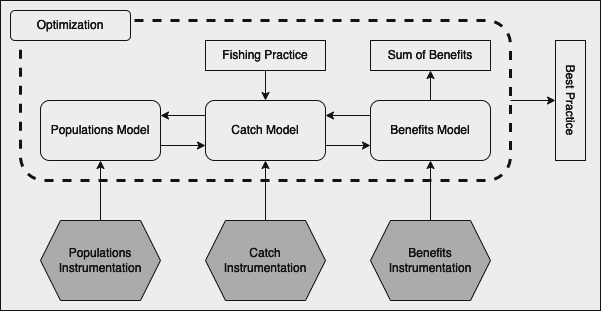
\includegraphics[width=\linewidth]{drawings/high_level_instrumentation.png}
  \caption{Instrumentation}
  \label{fig:high_level_instrumentation}
\end{figure}
\newline
\rule{\textwidth}{0.5pt} 
\vspace{5pt}

We've been talking about models quite flippantly. That's the nice thing about abstractions, you can talk about them as if they are but an arm's reach away, just ready to be plucked out of the mental sky of the imagination. Reality is rarely so kind. Models are monsters. Glorious to behold, tricky to master, and devilishly hard to train, they require significant expertise and thought to get right. But in and amongst all of their diversity there is one thing all models share - models must be fit.
\newline

Now by that I don't mean models need to be burly or able to run a race in a specific period of time, what I mean is that models have to fit in - you must look at them and see nothing but reality itself. And fitting a model is one of those things that while easy enough to explain is devilishly hard to do. 
\newline

So in the usual fashion, let's do the easy part - the explaining. 
\newline

Let's use a simple example. Fisheries scientists often have to model the relationship between age $t$ and length $L$. One one such model is the Von Bertalanffy growth curve:

$$L = L_{\infty}(1-e^{-Kt})$$

This equation is pretty straight forward. That exponential term, the $e^{-Kt}$, will, assuming $K>0$, go to zero as $t$ gets larger and larger. And that means that as the years go by $L$ becomes more and more like $L_{\infty}$. To put this more plainly growth starts out quickly and then slows down over time until it becomes barely perceivable, maxing out at this imaginary $L_{\infty}$ - the length of an infinitely old fish (who knows, perhaps some deity keeps pets). 
\newline

Whether or not you believe fish grow this way is irrelevant, it's just an illustration of fitting after all. And like all good simple examples it paints a nice clear point. The point is that this model, like all other models out there, has three main components - input variables - $t$, output variables - $L$, and parameters - $L_{\infty}$ and $K$. 
\newline

The way you use the model is also straightforward - you get some measurements, plug them into your input variables, run the equation, and get some predictions as the output variables. Easy peasy. 
\newline

There is a problem however - none of this is going to work if we don't know what $K$ and $L_{\infty}$ should be. This is where the fitting comes in. To build any model you have to have some situations in which both the input and output variables are known. Then you can choose the parameters that best fit that "ground truth" data. 
\newline

For example (I know, examples within examples!), suppose our measured ground truth looked something like Fig. \ref{fig:length_measurements_by_year}.
\newline


\begin{figure}[h!] 
  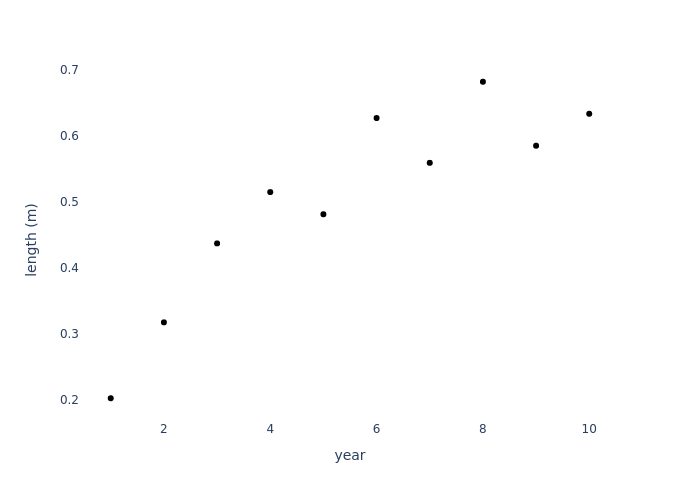
\includegraphics[scale=0.35]{notebooks/Fitting/new_measurements.png}
  \caption{Average Length Measurements by Year}
  \label{fig:length_measurements_by_year}
\end{figure}

First we can note that our measurements never exceed 0.7. So I'd say a pretty good guestimate for $L_{\infty}$ would be just that - 0.7.  Then we can try a few examples of $K$ and see what works well.
\newline

\begin{figure}[h!] 
  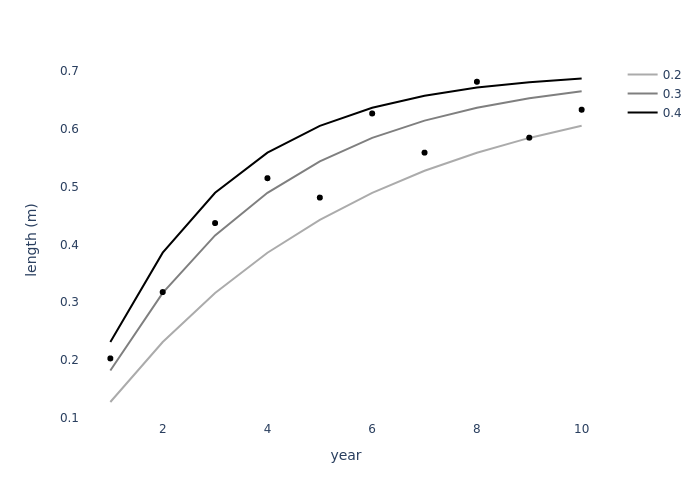
\includegraphics[width=\linewidth]{notebooks/Fitting/fit_lines.png}
  \caption{Attempting to Fit $K$}
  \label{fig:fitting_K}
\end{figure}

Fig. \ref{fig:fitting_K} shows us the predicted length vs year relationship for three values of $K$ - 0.2, 0.3, and 0.4. By just visual inspection we can see that 0.2 doesn't grow fast enough whereas 0.4 grows to quickly, so 0.3 is probably a reasonable fit.
\newline

How did I guess these? Well I built the example of course! Unfortunately we are rarely in possession of such retrospective knowledge and so mathematicians, scientists, and computer scientists have come up with loads of automated mechanisms for fitting parameters. (An absolutely fascinating subject by the way. If we had more time I would definitely nerd out about it). 
\newline

So in sum, to fit a model you need, ground truth data, a mechanism for arriving at the fit, and... well... the model is also pretty handy to have on hand. We have the model, folks have built the mechanisms for automatically tuning it, and so what's missing is the ground truth data. 
\newline

These data and the instrumentation and labor that goes into collecting it are the unsung heroes of the modeling world. Everyone loves to talk about the new artificial intelligence they just breathed life into, or how by switching models some prior, dubious assumptions could be relaxed, but none of that would be possible without the data. And that's why in my diagram they get their own special place.
\newpage

\noindent \rule{\textwidth}{0.5pt} 
\begin{figure}[h!] 
  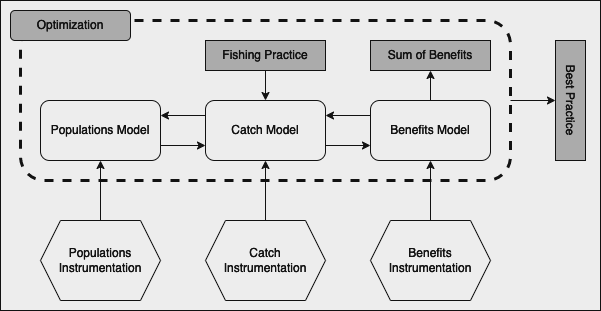
\includegraphics[width=\linewidth]{drawings/high_level_optimization.png}
  \caption{Optimization}
  \label{fig:high_level_optimization}
\end{figure}
\newline
\rule{\textwidth}{0.5pt} 
\vspace{5pt}

Voila! We've got ourselves some models that, thanks to our stunning ground truth data have been fit to look convincing like our earthly reality. Now what? Well to lean on my dodgy analogy from before, it's time to grab the steering wheel, hit the gas, and drive the fisheries mobile to a better tomorrow. To get a sense of what it's like to get behind the wheel let's once again turn to a simple(ish) example. 
\newline

All optimizations begin with taking the knobs we intend to turn and quantifying them. In our case, to keep things clear, we're going to assume that we're just directly controlling fishing mortality $F$ (and yes, I admit, I have no idea how you'd actually control such a thing directly). 
\newline

Next we know we need to start with our models and we may as well begin with the population side of things. Let the sweeping assumptions begin!
\newline

First we're going to assume that the fish population dies off in strict accordance to a mathematical equation (cold? I suppose so):

$$\frac{dN}{dt}=-ZN$$

How to read this? It just says that the \textit{instantaneous} decrease in fish is proportional to the number of fish present. $Z$ controls how rapidly death comes knocking. Make it large and the fish population collapses quickly, make it small and you'll get a lot of nice, old, wizardly fish. In general though fisheries scientists split $Z$ into $M$ and $F$ where $M$ is dubbed the "natural mortality". 
\newline

Our equation happens to be a pretty standard differential equation and therefore has a pretty standard solution:

$$N = N_0 e^{-Zt}$$

The next assumption we're going to make is that $F$ and $M$ don't really change year to year. This is nice because it means every generation of fish is exactly like all the others and so by studying one cohort we study them all. As such, the number of fish $t_y$ years old is simply the number of fish left in any single generation when that generation reachs $t_y$ years old:

$$N_y = N_0 e^{-Zt_y}$$

Alright, so much for our population modeling. On to the next!
\newline

For catch things are pretty simple. $F/Z$ represents what fraction of the fish sent to the afterlife ended up on someone's boat. So all we need to know is how many fished kicked the proverbial bucket and we'll be able to compute the size of the catch per age. If the overall fish mortality in an age class $D_y$ is given by:

$$D_y = N_{y-1} - N_y =N_0(e^{-Zt_{y-1}}- e^{-Zt_y})$$

Then the catch for that year class would be $C_y$:

$$C_y = \frac{F}{Z} D_y = \frac{FN_0}{Z}(e^{-Zt_{y-1}}- e^{-Zt_y})$$

And that's it, catch model complete (feel too easy? illustrations are wonderfully deceiving like that).
\newline

To complete our triad we need the benefits model. More generous assumptions on the way. First we're going to assume that no matter what we do the 0th year class (i.e. the babies) is always the same size. This obviously, is a wild assumption because if $F=1$ there'd by absolutely no fish to make those babies. However we're going to wave it off and assure ourselves as we make the historically dangerous assumption that $F\approx 1$ is impossible. The other assumption we're going to make is that the value of a fish is equal to the cube of its length. Basically we're treating a fish like a square, asserting that the volume of that square is the cube of one side, and then saying weight is equal to volume. Rather than fishing blobfish we're fishing blockfish. Crude, to be sure, but actually this is, practically speaking, a pretty reasonable line of thinking. The result? If we have length, we have weight, and if we have weight we have money. Bring in the Von Bertalanffy growth curve!

$$L_y = L_{\infty}(1-e^{-Kt_y})$$

Through a quick cubing operation this $L_y$ quickly translates into a weight and thus value $V_y$:

$$V_y = L_y^3C_y$$

Now remember this is per age class. In our simple example every age class is fished (requiring some pretty crazy, hyper adaptive nets) so the total value is:

$$V = \sum_y V_y$$

Alright let's put all this together into a final equation for fishery value $V$:

$$V = \sum_y \frac{FN_0}{F+M}(e^{-(F+M)t_{y-1}}- e^{-(F+M)t_y})(L_{\infty}(1-e^{-Kt_y}))^3$$

Next we know we need to split things into parameters, input values, and output values. $L_\infty$, $K$, $M$, and $N_0$ are all parameters and therefore need fitting, but otherwise $V$ is simply a function of $F$ - i.e we have but one input and output variable. So let's once again ignore anything remotely difficult and assume our parameters have already been fit to $L_\infty=1$, $K=0.1$, $M=0.1$, and $N_0=1$. What we get is Fig. \ref{fig:value_v_F}
\newline

\begin{figure}[h!] 
  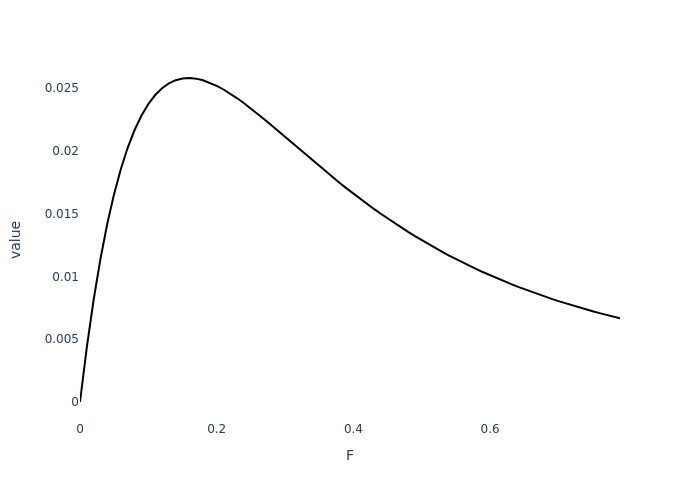
\includegraphics[width=\linewidth]{notebooks/SimpleOptimization/value_v_F.png}
  \caption{Value versus Fishing Mortality}
  \label{fig:value_v_F}
\end{figure}

And boom! This is why optimization is important. Start at $F=0$ and we get an obvious result - if you don't fish you don't get any fish (surprise!). Then as we begin to apply some fishing pressure $F>0$ we can see that the value starts rising rapidly - also expected. However something really interesting happens once we cross $F\approx 0.2$ the value starts to go down! Turns out there is such a thing as too much of a good thing. What's going on here is that after a certain point ramping up the fishing pressure starts to kill so many \textit{young} fish that fish aren't able to grow up into the big chonkers that bring much of the value of the fishery. As a result, the fishery actually becomes poorer as we put more effort into it! More effort screws up the demographics which in turn screws up the fishery. Pretty fascinating if you ask me.  
\newline

Alright, clearly this was a contrived example and part of what made it so easy was our "management" was parametrized by a single variable $F$. This meant that we could just plot out all of the options and choose the best one. In theory, this brute force approach always work. But theory and practice rarely agree on anything and tend to get in fisticuffs over things that were supposed to be the easy part. Practice, you see, suffers from the curse of dimensionality. 
\newline

To illustrate suppose you start with a single parameter case like ours, but one where the parameter is categorical (i.e. it takes on a specific set of values). Maybe that parameter can take on 10 values. This in turn means you need only search $10$ different cases to find your optimal case for sure. 
\newline

Alright, now suppose that you add another 10 value parameter. What comes next can be a little hard to grasp in the abstract, so let's suppose that our first parameter corresponds to the kind of gear used and the second to how many months folks can go out fishing. That means that for each selection of gear we have to independently try each selection of months. This means that rather than having ten cases we have ten times ten cases. Add another parameter (say catch limits per boat) and you now have ten times ten times ten or one thousand cases to check. You can probably see where this is going... in general with $N$ such parameters there are $10^N$ cases to explore!
\newline

This gets computationally inefficient really, really fast. So when folks optimize really large problems (with loads of parameters) they obviously have to turn to things besides brute force search.
\newline

Generally speaking there are two categories - analytic and meta-heuristic. While going into either would take up far too much room here the basic idea behind each is to use knowledge about the solutions you've already looked at to be clever about the next case you choose so you can quickly find better values without having to search the \textit{whole} space. However, nothing comes for free, and so this strategy has a drawback. A pretty darn significant drawback. Except for in a limited number of special cases, these faster strategies don't actually \textit{guarantee} optimality. Instead it's up to you to use them skillfully in order to make the likelihood of finding optimality more and more \textit{probable}. As such it's incredibly important to know what you're using quite intimately to avoid having the wool pulled over your eyes!
\newpage

\noindent \rule{\textwidth}{0.5pt} 
\begin{figure}[h!] 
  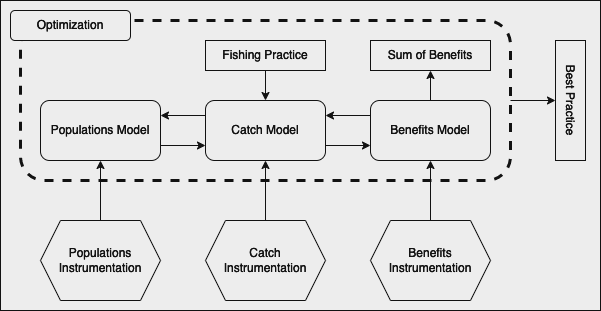
\includegraphics[width=\linewidth]{drawings/high_level.png}
  \caption{30,000ft View}
  \label{fig:high_level}
\end{figure}
\newline
\rule{\textwidth}{0.5pt} 
\vspace{5pt}

At this point we've covered a lot of ground. We've got models that drive our optimization, instrumentation creating the ground truth data used to fit those models, and the optimization itself. Put these together and you can start working toward finding the right set of fishing parameters to maximize the particular balance of benefits presently under consideration. 
\newline

However through all of that something should have become frighteningly clear - all of this is \textit{entirely} dependent on the models used. And so an obvious question comes walking, nay barging - existential sword in hand - through the door - what can go wrong with the modeling itself? We turn to that next. 
\newpage

\bibliographystyle{plain}
\bibliography{reference}
\end{document}